\documentclass[twocolumn]{aastex63}

% typography
\usepackage[T1]{fontenc}

\setlength{\parindent}{1.\baselineskip}
\newcommand{\acronym}[1]{{\small{#1}}}
\newcommand{\package}[1]{\textsl{#1}}
\newcommand{\gaia}{\textsl{Gaia}}
% \newcommand{\hst}{\textsl{HST}}
% \newcommand{\pans}{\textsl{Pan-STARRS}}

% \newcommand{\deg}{\ensuremath{\textrm{deg}}}
\newcommand{\msun}{\ensuremath{\textrm{M}_\odot}}
\newcommand{\myr}{\ensuremath{\textrm{Myr}}}
\newcommand{\gyr}{\ensuremath{\textrm{Gyr}}}
\newcommand{\kpc}{\ensuremath{\textrm{kpc}}}
\newcommand{\kms}{\ensuremath{\textrm{km}\,\textrm{s}^{-1}}}
\newcommand{\masyr}{\ensuremath{\textrm{mas}\,\textrm{yr}^{-1}}}
\newcommand{\feh}{\ensuremath{\textrm{[Fe/H]}}}
\newcommand{\afe}{\ensuremath{\textrm{[$\alpha$/Fe]}}}
\newcommand{\changes}[1]{{\textbf{#1}}}
\hyphenation{kruijs-sen}

% aastex parameters
% \received{not yet; THIS IS A DRAFT}
%\revised{not yet}
%\accepted{not yet}
% % Adds "Submitted to " the argument.
% \submitjournal{ApJ}
\shorttitle{}
\shortauthors{bonaca \& kruijssen}

%@arxiver{}
\usepackage{amsmath}

\begin{document}\sloppy\sloppypar\raggedbottom\frenchspacing % trust me

\title{The low masses of globular clusters that dissolved in the Milky Way}

\correspondingauthor{Ana~Bonaca}
\email{ana.bonaca@cfa.harvard.edu}

\author[0000-0002-7846-9787]{Ana~Bonaca}
\affil{Center for Astrophysics | Harvard \& Smithsonian, 60 Garden Street, Cambridge, MA 02138, USA}

\author[0000-0002-8804-0212]{J.~M.~Diederik~Kruijssen}
\affiliation{Astronomisches Rechen-Institut, Zentrum f\" ur Astronomie der Universit\" at Heidelberg, M\" onchhofstra\ss e 12-14, D-69120 Heidelberg, Germany}
\affil{Center for Astrophysics | Harvard \& Smithsonian, 60 Garden Street, Cambridge, MA 02138, USA}


\begin{abstract}\noindent % trust me
Numerous stellar streams that have been discovered in the Milky Way as evaporated globular clusters show signs of dynamical perturbation.
N-body models that can illuminate the origin of these perturbations require the cluster's initial mass as a fundamental input parameter.
Here we present orbits and masses of 20 dissolved globular clusters in the Milky Way.
We constrained the streams' orbits by fitting the 3D positions of a stream's endpoints from ground-based photometry and its proper motions from Gaia.
Assuming a dissolution time of 10\,Gyr, we use orbital apocenters and eccentricities to estimate the clusters' initial mass.
Disrupted globular clusters have preferentially lower masses than the surviving population, with the median mass being an order of magnitude smaller.
The overall distribution of apocenters and eccentricities is similar for the disrupted and surviving clusters, however, at a fixed mass disrupted clusters have smaller apocenters and larger eccentricities.
The progenitors of tidal streams observed at the present are a specific, low-mass subset of the initial globular cluster population.
This has implications for establishing the role of internal dynamics in sculpting the observed tidal debris, and the amount of external perturbation, e.g., from dark-matter subhalos, that these streams experienced.
\end{abstract}

\section{Introduction}
\label{sec:intro}

Theoretical studies of globular cluster dynamics predicted that stars escape globular clusters due to two-body relaxation and tidal stripping \citep[e.g.,][]{spitzer:1987, baumgardt03}, forming long and thin tidal tails along the cluster's orbit \citep{combes:1999}.
Such tidal tails were first detected around the Palomar~5 globular cluster \citep{odenkirchen:2001, rockosi:2002}.
Stellar streams of similar width and length, but without a surviving progenitor, have been discovered throughout the Milky Way \citep[e.g.,][]{gd:2006, grillmair:2009, bonaca:2012, shipp:2018, ibata:2019}, likely constituting a population of completely dissolved globular clusters.

Forming kinematically cold and being shaped by the Milky Way tides, we expect that globular cluster streams are sensitive both to the global distribution of matter in the Galaxy \citep[e.g.,][]{lux:2013, bonaca:2014, sanders:2014}, and to small-scale perturbations, such as predicted from low-mass dark-matter subhalos \citep[e.g.,][]{ibata:2002, yoon:2011, erkal:2016}.
Detailed observations have recently revealed signatures of perturbation in a number of thin streams \citep[e.g.,][]{pwb, bonaca:2019a, bonaca:2020, li:2020}, which may be attributed to impacts of dark-matter subhalos \citep[e.g.,][]{bonaca:2019b, banik:2019}.
Alternatively, the observed features may be due to the way stars escape globular clusters \citep[e.g.,][]{kuepper:2008, kuepper:2010} or due to the onset of cluster disruption before its original host galaxy accreted onto the Milky Way \citep[e.g.,][]{carlberg:2018, malhan:2020}.

To employ tidal tails as cosmological tracers of dark matter, it is essential to disentangle the internal and external sources of perturbation.
Direct N-body simulations of the progenitor globular clusters in realistic environments would accurately capture the relevant processes \citep[e.g.,][]{renaud:2015}.
However, these simulations remain out of reach because a cluster's dynamical evolution sensitively depends on its mass \citep[e.g.,][]{hh:2003, balbinot:2018}, and masses of most dissolved clusters are extremely uncertain \citep[e.g.,][]{erkal:2016b}.

Our goal in this Letter is to dynamically estimate masses of disrupted globular clusters that are now observed as stellar streams in the Milky Way.
The timescale for cluster disruption is determined by its initial mass (more massive clusters take longer) and its orbit: clusters on more eccentric orbits and with smaller apocenters dissolve faster \citep{kruijssen09}.
Using data from the Gaia mission \citep{gdr2}, we determine stream orbits in Section~\ref{sec:orbits}.
Since the streams are coherent, we assume the progenitor globular clusters disrupted recently \citep{helmi:2003}, and in Section~\ref{sec:disrupted} calculate their masses.
We close by discussing the implications of the inferred low masses for dynamical studies of stellar streams, and place this population of disrupted globular clusters in the context of cluster and galaxy formation.


\section{Stream Orbits}
\label{sec:orbits}
A total of x thin stellar streams, likely disrupted globular clusters, have been reported in the Milky Way \citep[an up-to-date list is available in the \package{galstreams} package,][]{mateu:2018}.
Tidal debris from evaporating globular clusters nearly delineates the progenitor's orbit \citep[e.g.,][]{kupper:2012}, however, kinematic information is essential for accurate stream modeling \citep{bh:2018}.
Here we analyze a subset of y stellar streams with published proper motions (Table~\ref{table:streams}).

\begin{figure*}
\begin{center}
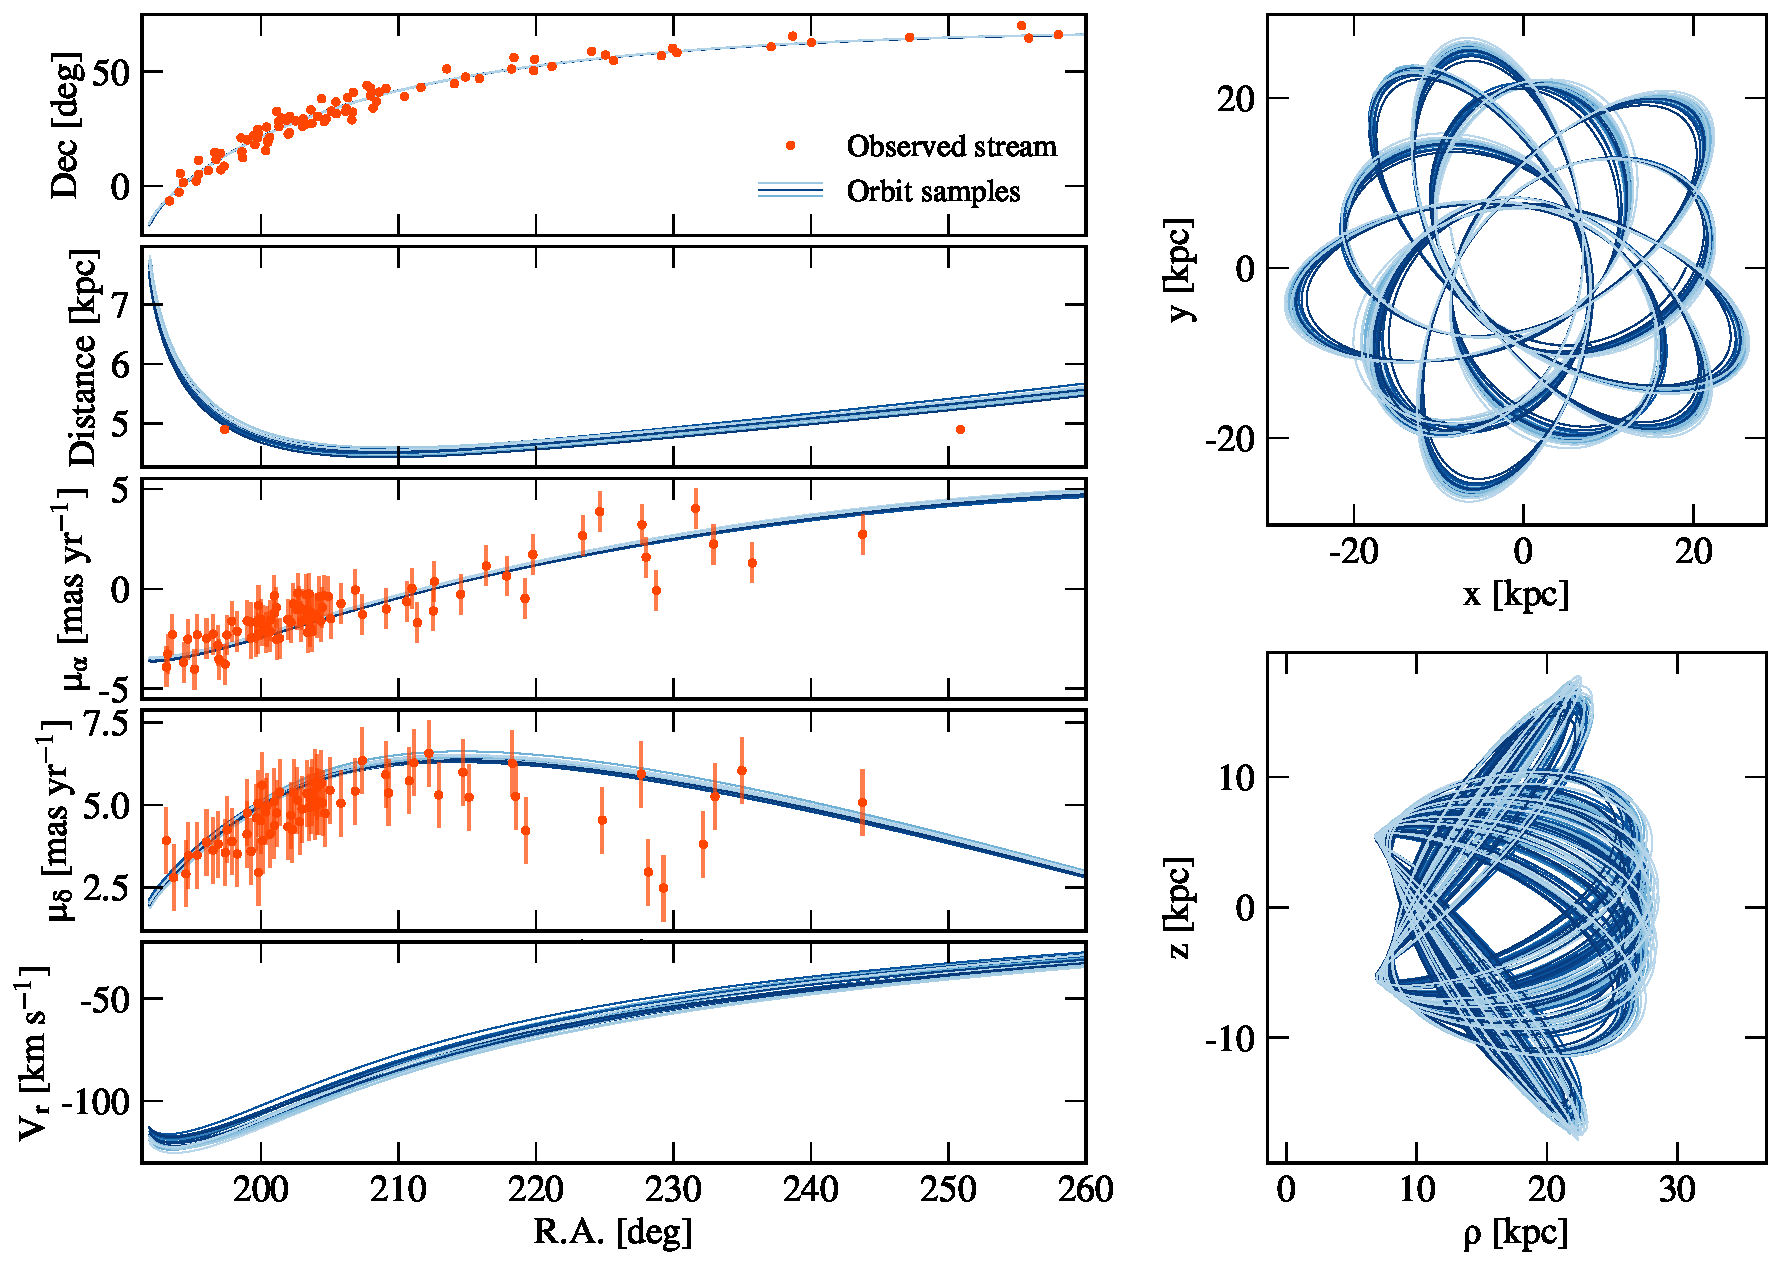
\includegraphics[width=0.9\textwidth]{figures/stream_fitting.pdf}
\end{center}
\caption{Orbital constraints for the Fj\"{o}rm stellar stream in the observed coordinates (left: panels from top to bottom show declination, distance, and proper motion components as a function of right ascension) and cylindrical Galactocentric coordinates (right: in and out of the Galactic plane for the top and bottom panels, respectively).
Different shades of blue represent orbit samples from the posterior constrained by the stream endpoints (orange points).
Current observations allow for a range of orbital apocenters and eccentricities.
}
\label{fig:streams}
\end{figure*}

We measure orbital parameters for a population of dissolved globular clusters by fitting orbits to sky positions, distances, and proper motions of stream endpoints.
Due to limited observational data on some streams, we decided to fit only the stream endpoints to ensure a homogeneous treatment of the entire sample.
\citet{riley:2020} demonstrated that the 3D positions of stream end-points robustly constrain their orbital poles, while \citet{ibata:2019} found that the absence of radial velocities produces no significant biases in orbit determination for streams with proper motion data.
Therefore, we expect our strategy of recovering orbits from 5D positions of stream endpoints to perform well.
In Section~\ref{sec:discussion} we discuss how orbital constraints change for streams where additional data is available.
The endpoint sky positions and distances \citep{riley:2020}, and proper motions \citep[][as noted]{ibata:2019, shipp:2019} are listed in Table~\ref{table:streams}, along with the associated uncertainties.
Figure~\ref{fig:streams} shows these data for three representative streams as large black points (top to bottom: x, y, z).

We fit stream orbits in a three-component model of the Milky Way gravitational potential implemented in the \package{gala} package \citep{gala} and featuring a \citet{mn:1975} disk (mass: $5.5\times10^{10}\rm\, M_\odot$, scale-length: 3\,kpc, scale-height: 28\,pc), a \citet{hernquist:1990} bulge (mass: $4\times10^9\rm\, M_\odot$, scale-radius: 1\,kpc), and a \citet{nfw:1997} halo (scale-mass: $7\times10^{11}\rm\, M_\odot$, scale-radius: 15.62\,kpc, $z$-axis flattening: 0.95).
Similar to the orbit-fitting procedure of \citet{pwb}, we represent the orbit as a 6D location in phase-space, fixing its right ascension, R.A., and solving for the remaining 5D coordinates (declination, distance, radial velocity, two proper motion components).
At the R.A. of the stream endpoints, we evaluate the orbital declinations, distances and proper motions against the observations, assuming Gaussian uncertainties.
The orbits are initialized at one of the stream endpoints, with a radial velocity such that the total velocity vector equals the circular velocity at that Galactocentric distance and points to the other endpoint.
We employ only minimal priors by requiring a bound orbit and the absolute radial velocity lower than 500\,\kms.

We begin the search for well-fitting stream orbits by maximizing the likelihood of orbits passing through the observed endpoints using the \package{scipy} implementation of the BFGS algorithm.
Focusing on this best-fitting solution, we further sample the likelihood with an affine-invariant sampler \package{emcee} to estimate the posterior distribution of the orbital parameters.
We advanced 64 walkers for 512 steps and kept the last 256 steps which converged to constant median and dispersion values for all model parameters.
The median, 16th and 84th percentiles of the constrained 5D coordinates are reported for each stream's orbit in Table~\ref{table:constraints}.

To visualize and further explore the streams' orbits, we randomly sampled 1,000 points from the posterior distributions of every stream (available at the project repository\footnote{\url{https://github.com/abonaca/disrupted_gc}}).
First, we integrated short orbital segments starting from these initial positions, and plot them as thin, black lines in the observable coordinates in Figure~\ref{fig:streams}.
For all of the streams, we recovered a class of orbital solutions that fits the observed stream endpoints.
The allowed spread in orbits is directly related to the observational uncertainties, so future improvements in distance and proper-motion measurements should further refine the orbital constraints.

To estimate current constraints on the orbital apocenter, $r_{apo}$, and eccentricity, $e=(r_{apo} - r_{peri})/(r_{apo} + r_{peri})$, we additionally performed 5\,Gyr long orbit integrations starting from the same initial positions.
These longer orbits are shown in cylindrical Galactocentric coordinates in the right panels of Figure~\ref{fig:streams} (different colors correspond to different samples from the posterior distribution).
- comment on precision
In Table~\ref{table:constraints} we report the median, 16th and 84th percentiles of the orbital apocenter and eccentricity, while in the next section we estimate the progenitor masses using the samples directly to fully account for correlations between these orbital parameters.

- caveats:
-- orbit fits -> compare to published ones
-- stream ne orbit


\section{Masses of Disrupted globular clusters}
\label{sec:disrupted}

We estimate the masses of the globular clusters producing the streams using a simple analytic globular cluster disruption model \citep{lamers05}, which reproduces direct $N$-body simulations of globular clusters undergoing tidal evaporation in a static background potential \citep{baumgardt03}. Specifically, we obtain a `pre-evaporation' globular cluster mass $M_0$ by estimating the total mass loss due to stellar evolution and tidal evaporation for a cluster on the inferred orbit over some timescale $t$. We refrain from deriving an `initial' globular cluster mass, because tidal evaporation in the host galaxy halo is not the only mass loss mechanism experienced by globular clusters over the course of their history. Prior to being deposited into the halo, globular clusters were disrupted by tidal shocks due to gravitational perturbations from overdensities in the interstellar medium of their natal galaxy \citep[e.g.][]{gieles06,kruijssen11,miholics17,pfeffer18}. Integrated over the history of globular clusters, tidal shocks are thought to dominate the total dynamical mass loss \citep[e.g.][]{kruijssen15b}. Therefore, the quantity $M_0$ refers strictly to the `pre-evaporation' globular cluster mass -- after the first phase of disruption tidal shocks, but before the second phase of disruption by tidal evaporation. We also include the total amount of mass lost by stellar evolution, so that only the mass loss by tidal shocks is unaccounted for.

We relate $M_0$ to the orbit of the stellar stream by assuming a present-day globular cluster mass of zero (consistent with the fact that only a fossil stream remains) and writing eq.~7 of \citet{lamers05} as
\begin{equation}
\label{eq:m0}
M_{\rm 0}=\frac{1}{\mu_{\rm ev}(t)}\left(\frac{\gamma t}{t_0}\right)^{1/\gamma} .
\end{equation}
In this expression, $\mu_{\rm ev}(t)$ is the fraction of the initial globular cluster mass lost by stellar evolution, provided by \citet{lamers05} as
\begin{equation}
\label{eq:muev}
\mu_{\rm ev}(t)=1-q_{\rm ev} ,
\end{equation}
with
\begin{equation}
\label{eq:qev}
\log_{10}{q_{\rm ev}}(t) = [\log_{10}(t/{\rm yr})-a_{\rm ev}]^{b_{\rm ev}}+c_{\rm ev} ,
\end{equation}
and $a_{\rm ev} = 6.93$, $b_{\rm ev} = 0.255$, and $c_{\rm ev} = -1.682$, appropriate for a GC-like metallicity of $0.02{\rm Z}_\odot$ and a \citet{kroupa01} stellar initial mass function \citep{kruijssen08}. The variables $\gamma$ and $t_0$ represent the exponent and proportionality factor, respectively, of the Lamers cluster disruption law:
\begin{equation}
\label{eq:lamers}
\tau_{\rm dis}=t_0\left(\frac{M}{\msun}\right)^\gamma ,
\end{equation}
where $\tau_{\rm dis}$ is the cluster disruption timescale. We follow \citet{kruijssen09} in adopting $\gamma=0.7$ and relating $t_0$ to the orbital parameters as
\begin{equation}
\label{eq:t0}
t_0 = t_{0,\odot}\left(\frac{R_{\rm a}}{8.5~\kpc}\right)\left(\frac{v_{\rm c}}{220~\kms}\right)^{-1}(1-e) ,
\end{equation}
with $t_{0,\odot}=10.7~\myr$ and $R_{\rm a}$, $v_{\rm c}$, and $e$ denoting the orbital apocenter radius, circular velocity, and orbital eccentricity, respectively. Finally, we assume that the time spent by each globular cluster orbiting the Milky Way prior to dissolving into a fossil stream is $t=10~\gyr$. This is motivated by the typical ages of globular clusters in the Galactic halo \citep[$\sim12~\gyr$, e.g.][]{kruijssen19e} and by recent results showing that fossil stream lifetimes are much shorter than globular cluster ages (!!REF), such that the progenitors of fossil streams must have disrupted in the past few Gyr. Our results are robust to this choice -- an error of 0.3~dex (i.e.\ a factor of 2) in $t$ translates into an error of just 0.2~dex in the pre-evaporation mass $M_0$.

\begin{figure*}
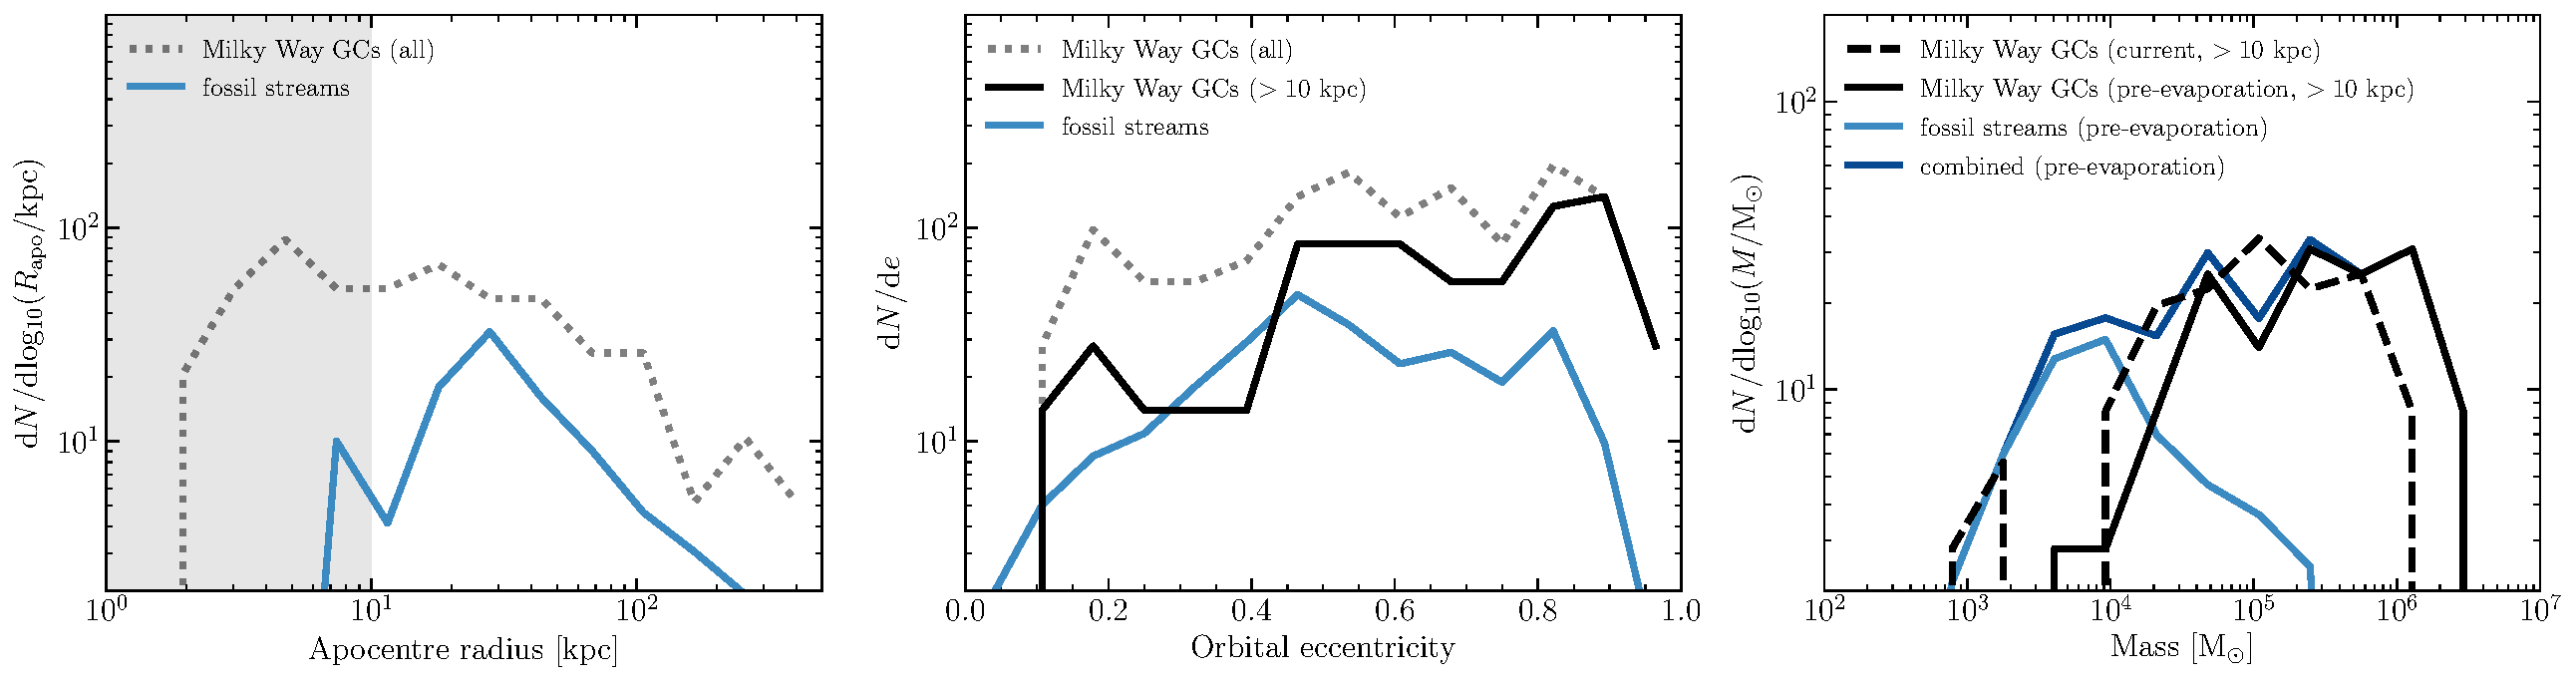
\includegraphics[width=\hsize]{figures/distributions_mc.pdf}%
\caption{
\label{fig:hist}
Demographics of fossil streams (and their progenitor clusters) compared to those of the Galactic globular cluster population. Left: Apocentre radius distributions. The gray-shaded area indicates the inner radii ($\leq10$~kpc) where few fossil streams are found. In the middle and right panels, we therefore consider the globular clusters outside of these radii. Middle: Orbital eccentricity distributions. globular clusters have a weak excess of high eccentricities relative to fossil streams. Right: Mass distributions, both for current globular clusters and for the masses of fossil streams and globular clusters after rewinding their evaporation-driven mass loss in the Galactic halo. The progenitors of fossil streams were systematically a factor of $>10$ less massive than globular clusters.}
\end{figure*}	
We propagate the uncertainties on the fossil streams' orbital parameters into those on the pre-evaporation masses by applying eq.~(\ref{eq:m0}) to the entire sample of MCMC solutions. The resulting distributions of all apocenter radii, eccentricities, and pre-evaporation masses of the fossil streams in the MCMC sample are shown in \autoref{fig:hist}, where we also include the population statistics of Galactic globular clusters that have survived till the present day. For these surviving globular clusters, we also include an estimate of their pre-evaporation masses.

\begin{figure*}
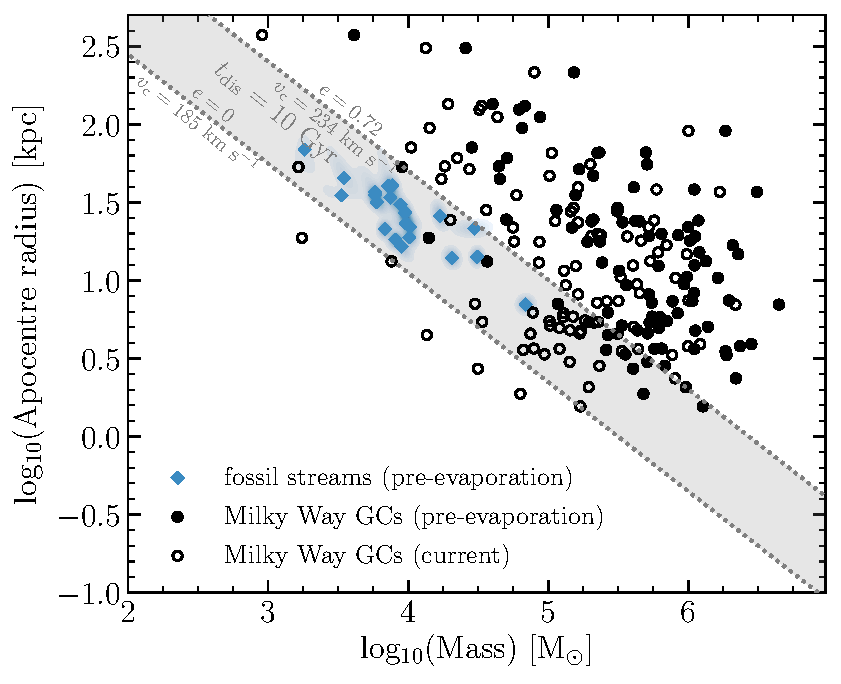
\includegraphics[width=0.5\hsize]{figures/mass_rapo.pdf}\\
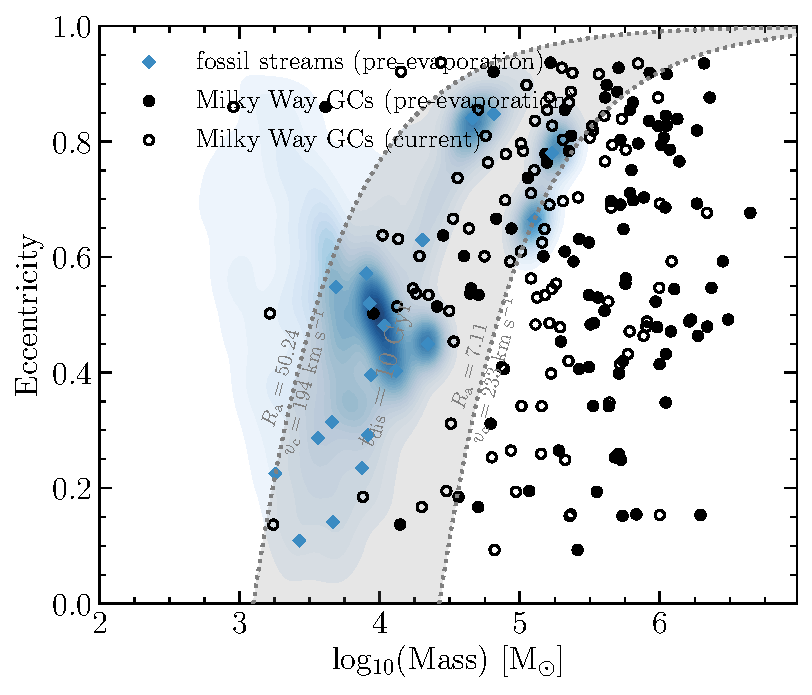
\includegraphics[width=0.5\hsize]{figures/mass_ecc.pdf}%
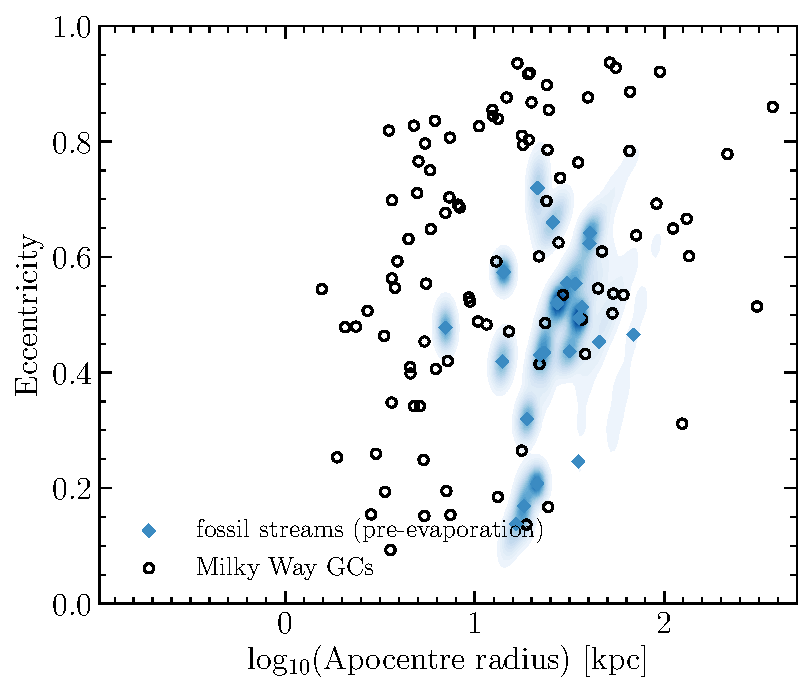
\includegraphics[width=0.5\hsize]{figures/rapo_ecc.pdf}%
\caption{
\label{fig:kde}
Two-dimensional demographics of fossil streams progenitors compared to those of the Galactic globular cluster population. Top left: Mass-apocentre radius plane. Bottom left: Mass-eccentricity plane. Bottom right: Apocentre radius-eccentricity plane. In each panel, the contours show a two-dimensional Gaussian kernel density estimate for the fossil stream progenitors, using the complete sample of MCMC realizations. Blue symbols show the best-fitting result for each fossil stream. Open black symbols show current globular clusters, whereas filled black symbols show their pre-evaporation masses, i.e.\ those corrected for evaporation-driven mass loss on their current orbits. In each panel, the gray-shaded band shows the range in each panel that is predicted to be occupied by the fossil stream progenitors assuming 10~Gyr of evolution, given their range of orbital properties and progenitor masses (indicated by the annotations in gray). The fossil stream progenitors are generally clearly offset from the globular clusters.}
\end{figure*}


\section{Discussion}
\label{sec:discussion}

\begin{figure}
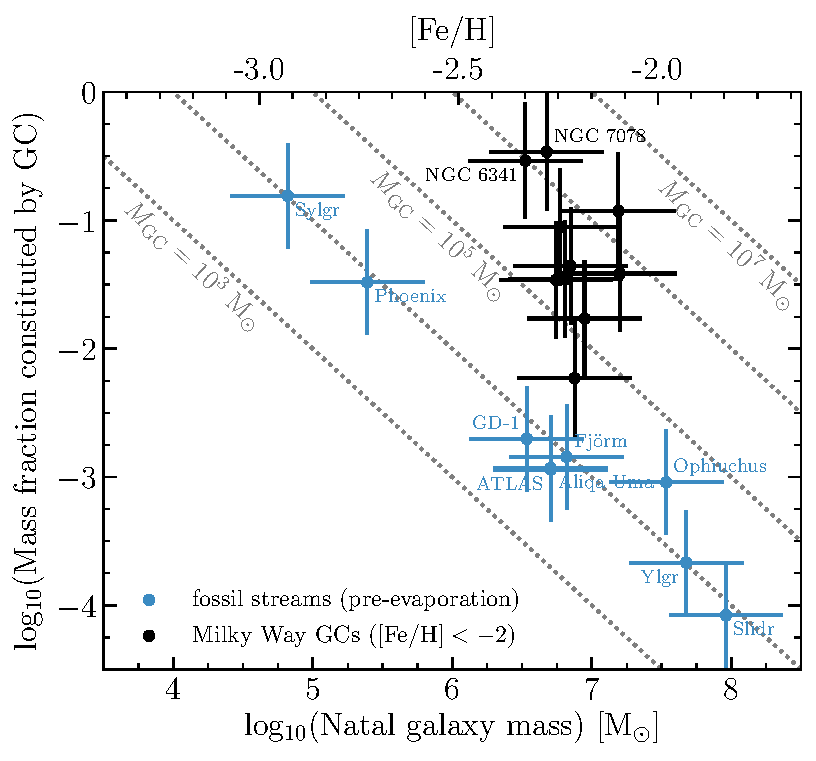
\includegraphics[width=\hsize]{figures/mhost_fraction.pdf}%
\caption{
\label{fig:mhost}
Mass fraction of the natal galaxy constituted by the progenitors of fossil streams and globular clusters (with ${\rm [Fe/H]}<-2$) as a function of the natal galaxy mass. The sample is restricted to fossil streams with known metallicities, which are converted to a natal galaxy mass using the galaxy mass-metallicity relation between $z=3$ and $z=6$. Error bars combine metallicity uncertainties with the evolution of the mass-metallicity relation across this redshift range. On average, fossil stream progenitors constituted a smaller fraction of their natal galaxy's mass than globular clusters, but the progenitors of the most metal-poor fossil streams likely represented a significant fraction of the lowest-mass galaxies ever to exist.}
\end{figure}

We determined orbits of 20 globular clusters disrupted in the Milky Way by fitting sky positions, distances, and proper motions of the remnant stellar streams.
Assuming that the progenitor clusters dissolved recently, we integrated the orbit-dependent mass-loss rate to infer their pre-evaporation masses.
The orbital distribution of disrupted globular clusters, in particular their apocenters and eccentricities, is similar to the orbital properties of the surviving population.
However, the inferred masses of disrupted globular clusters peak at $10^4\,\msun$---significantly lower than the mass of a typical globular cluster in the Milky Way today.
In this section we discuss this population of low-mass, disrupted globular clusters as tracers of both the Galactic gravitational potential and early star formation, and conclude with an outlook for future follow-up studies.

% * summary
% - used gaia data on 20 thin stellar streams, presumed disrupted globular clusters, to fit their orbits
% - found similar distribution of apocenters and eccentricities to surviving gc beyond 10kpc
% - inferred disrupted gc masses peaking at $10^4\,\msun$, lower than the surviving population
% - however, the most metal-poor clusters may have been a significant fraction of the host galaxy's stellar mass at the formation time
% - here: caveats, implications for streams as tracers of the mw potential, implications for studies of globular clusters as a population


* implications for individual streams
- compare to mass estimates in the detect part of the stream -> are they mostly detected or are they extending past the currently detected endpoints?
- hyades tails discovered -> is there a mass gap -> more streams to be discovered?
- lower mass -> implications for epicycles

* population-level inference
- low mass, recently disrupted, would expect to detect w jwst?
--> more numerous gc in the past, relation to clumpy disks at high z?
--> if the total count used to estimate the halo mass at high z, would need to be calibrated?
- low mass, but if mdf the same as host, those at low metallicity are a high fraction of the host galaxy mass
--> window into the lowest mass, most dm dominated galaxies

* future improvements:
- mass function slope -- do we understand why flat?
--> not interpretable at the moment, as the stream census incomplete; if it were complete, we could recover the ism-disruption stage mass-function
--> useful for understanding star formation, especially in low-metallicity regime, relevant for reionization?
-- progenitor: gc or dwarf? reasonably certain these are gc, but ideally to be confirmed w the presence of funky abundances (eg Hansen)
-- complete census
% do it in section -- 10 Gyr disruption time for estimating the mass + other systematics (estimate these sources of uncertainty)
-- many spec surveys coming online, potential to discover all streams (the ones in gaia less coherent than those discovered photometrically) and get their metallicities


\vspace{0.5cm}
It is a pleasure to thank:

\software{
\package{Astropy} \citep{astropy, astropy:2018},
\package{gala} \citep{gala},
\package{IPython} \citep{ipython},
\package{matplotlib} \citep{mpl},
\package{numpy} \citep{numpy},
\package{scipy} \citep{scipy}
}

\bibliographystyle{aasjournal}
\bibliography{disrupted_gc}


\end{document}


